% ===================== Lattice QCD (thesis Ch. 3, with 2023 slides) =====================
\section{Lattice QCD}

% Slide 9
\begin{frame}{Lattice QCD: links, plaquette and the Wilson action}
  \begin{columns}[c]
    \begin{column}{0.42\textwidth}
      \begin{itemize}
        \item Euclidean grid $\Lambda_4$ with spacing $a$. Quarks on sites; gluons as links $U_\mu(x)=e^{iaA_\mu(x)}\in SU(3)$.
        \item Plaquette:
      \end{itemize}
      \[ P_{\mu\nu}(x)=U_{\mu}(x)\,U_{\nu}(x+\hat{\mu})\,U^{\dagger}_{\mu}(x+\hat{\nu})\,U^{\dagger}_{\nu}(x) \]
      \begin{itemize}
        \item Wilson gauge action:
      \end{itemize}
      \[ \begin{aligned} S_{G}&=\frac{2}{g^2}\sum_{x}\sum_{\mu<\nu}\mathrm{Re}\,\Tr\big[1-P_{\mu\nu}(x)\big] \\ &= \frac{a^4}{2g^2}\sum_{x}\sum_{\mu,\nu}\Tr\big[F_{\mu\nu}^2\big]+\mathcal{O}(a^2) \end{aligned} \]
      \begin{itemize}
        \item Quarks: Wilson--clover fermions (removes doublers, $\mathcal O(a)$ improvement).
      \end{itemize}
    \end{column}
    \begin{column}{0.56\textwidth}
      \centering
      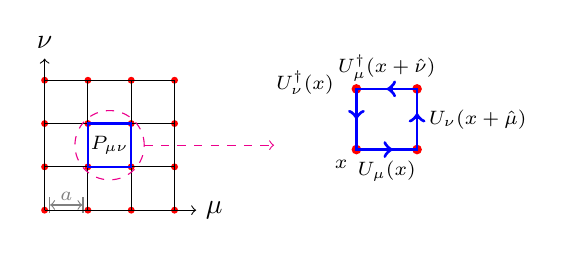
\begin{tikzpicture}[scale=0.55]
        \foreach \x in {0, 1, 2, 3} \foreach \y in {0, 1, 2, 3} \fill[red] (\x, \y) circle (0.08);
        \draw[|<->|, gray] (0.1, 0.12) -- (0.9, 0.12);
        \node at (0.5, 0.32) {\textcolor{gray}{\scriptsize $a$}};
        \foreach \x in {0, 1, 2, 3} \foreach \y in {0, 1, 2} \draw (\x, \y) -- (\x, \y + 1);
        \foreach \x in {0, 1, 2} \foreach \y in {0, 1, 2, 3} \draw (\x, \y) -- (\x + 1, \y);
        \draw[thick, blue] (1, 1) -- (2, 1) -- (2, 2) -- (1, 2) -- cycle;
        \node at (1.5, 1.5) {\scriptsize $P_{\mu\nu}$};
        \draw[->] (0, 0) -- (3.5, 0) node[right] {$\mu$};
        \draw[->] (0, 0) -- (0, 3.5) node[above] {$\nu$};
        \draw[magenta, dashed] (1.5, 1.5) circle (0.8);
        \draw[->, magenta, dashed] (2.3, 1.5) -- (5.3, 1.5);
        \begin{scope}[xshift=5.8cm, scale=1.4]
          \foreach \x in {1, 2} \foreach \y in {1, 2} \fill[red] (\x, \y) circle (0.08);
          \draw[thick, blue] (1, 1) -- (2, 1) -- (2, 2) -- (1, 2) -- cycle;
          \draw[blue,->, line width=1.2pt] (1.5, 1) -- ++(0.1,0);
          \draw[blue,<-, line width=1.2pt] (1.5, 2) -- ++(0.1,0);
          \draw[blue,->, line width=1.2pt] (2, 1.5) -- ++(0,0.1);
          \draw[blue,<-, line width=1.2pt] (1, 1.5) -- ++(0,0.1);
          \node at (0.75, 0.75) {\scriptsize $x$};
          \node at (1.5, 0.65) {\scriptsize $U_{\mu}(x)$};
          \node at (3.0, 1.5) {\scriptsize $U_{\nu}(x+\hat{\mu})$};
          \node at (1.5, 2.35) {\scriptsize $U^{\dagger}_{\mu}(x+\hat{\nu})$};
          \node at (0.15, 2.1) {\scriptsize $U^{\dagger}_{\nu}(x)$};
        \end{scope}
      \end{tikzpicture}
    \end{column}
  \end{columns}
\end{frame}

\begin{frame}{The elementary plaquette in the thesis}
  \centering
  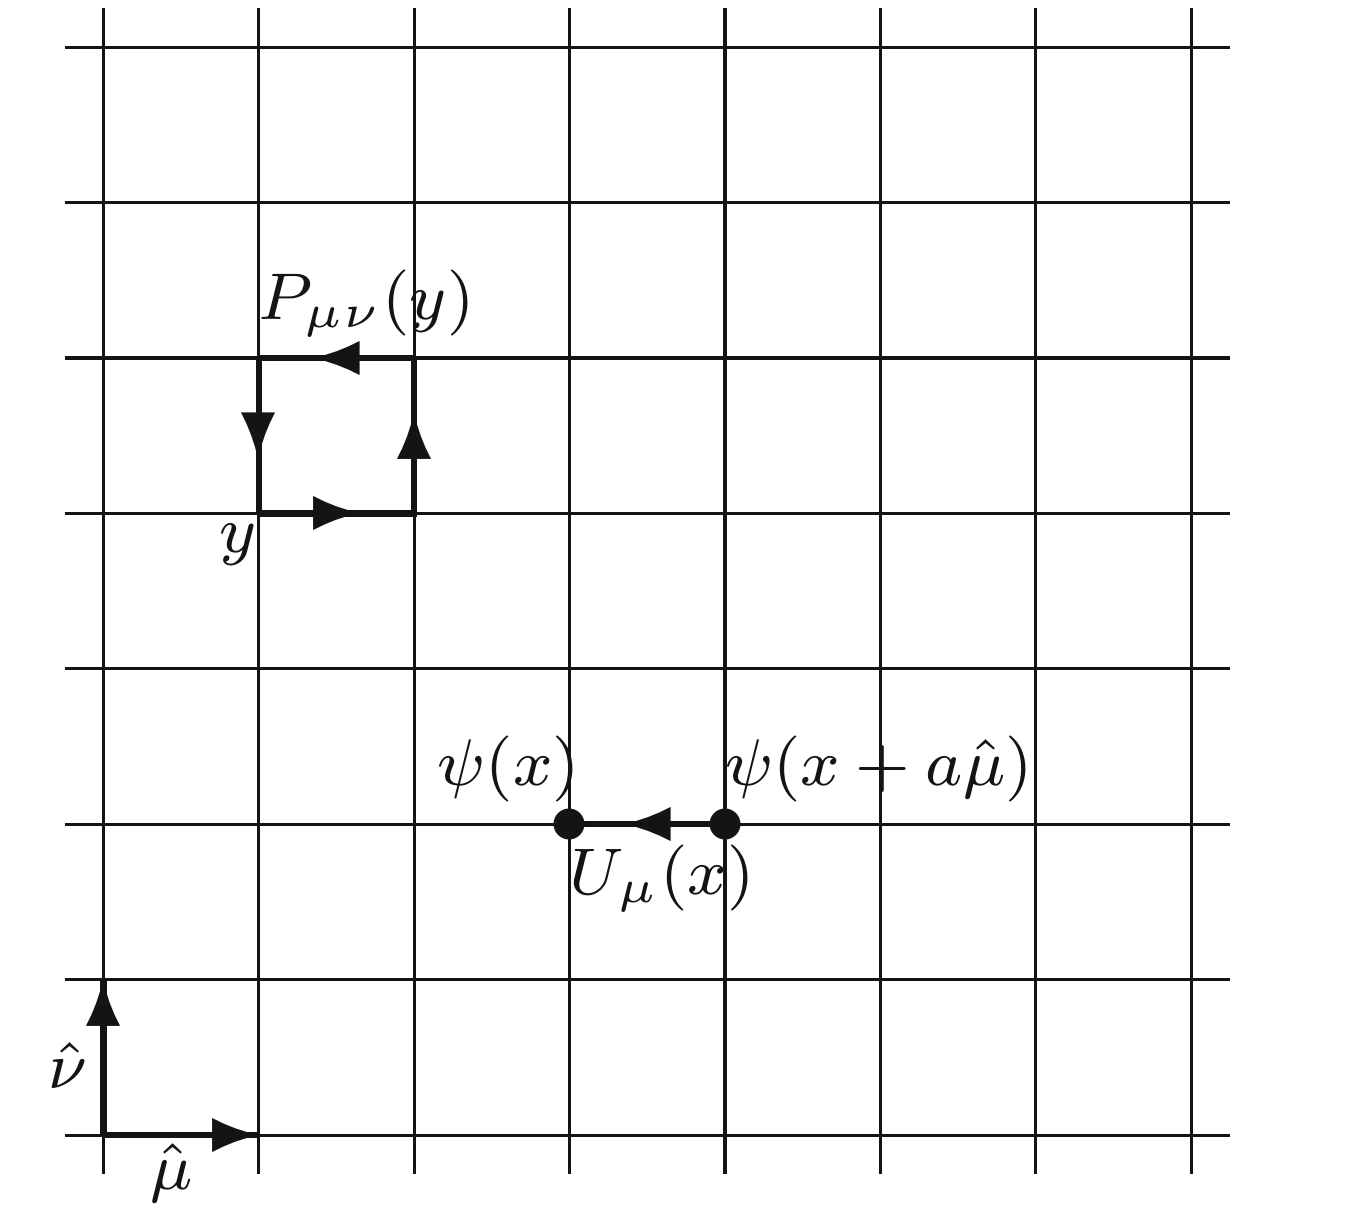
\includegraphics[width=.62\linewidth,height=.65\textheight,keepaspectratio]{LM_fig1_1_plaquette.png}
  \[
   P_{\mu\nu}(x)=U_\mu(x)U_\nu(x+\hat\mu)
                 U_\mu^\dagger(x+\hat\nu)U_\nu^\dagger(x).
  \]
  \figsrc{Thesis, Lattice QCD methodology, original plaquette figure.}
\end{frame}

% Slide 10
\begin{frame}{Path integral, Wick contractions and Monte Carlo}
  \quick
  \begin{columns}[c]
    \begin{column}{0.55\textwidth}
      \begin{itemize}
        \item Observables as Euclidean path integrals:
      \end{itemize}
      \[ \langle \mathcal{O} \rangle =\frac{\int \mathcal{D}[U]\mathcal{D}[\psi]\mathcal{D}[\bar{\psi}]\ \mathcal{O}\ e^{-S_{G}[U]-\bar{\psi}\mathcal{M}[U]\psi}}{\int\mathcal{D}[U]\mathcal{D}[\psi]\mathcal{D}[\bar{\psi}]\ e^{-S_{G}[U]-\bar{\psi}\mathcal{M}[U]\psi}} \]
      \begin{itemize}
        \item Integrating out the Grassmann quark fields gives $\det\mathcal{M}$ and \textbf{Wick contractions}: quark pairs become propagators $S=\mathcal{M}^{-1}$.
        \item Monte Carlo: sample configurations $U_n$ with probability $\propto \prod_f\det\mathcal M_f\; e^{-S_G[U]}$:
      \end{itemize}
      \[ \langle \mathcal O\rangle \approx \frac{1}{N}\sum_{n=1}^{N} \widetilde{\mathcal O}[U_n] \]
    \end{column}
    \begin{column}{0.43\textwidth}
      \centering
      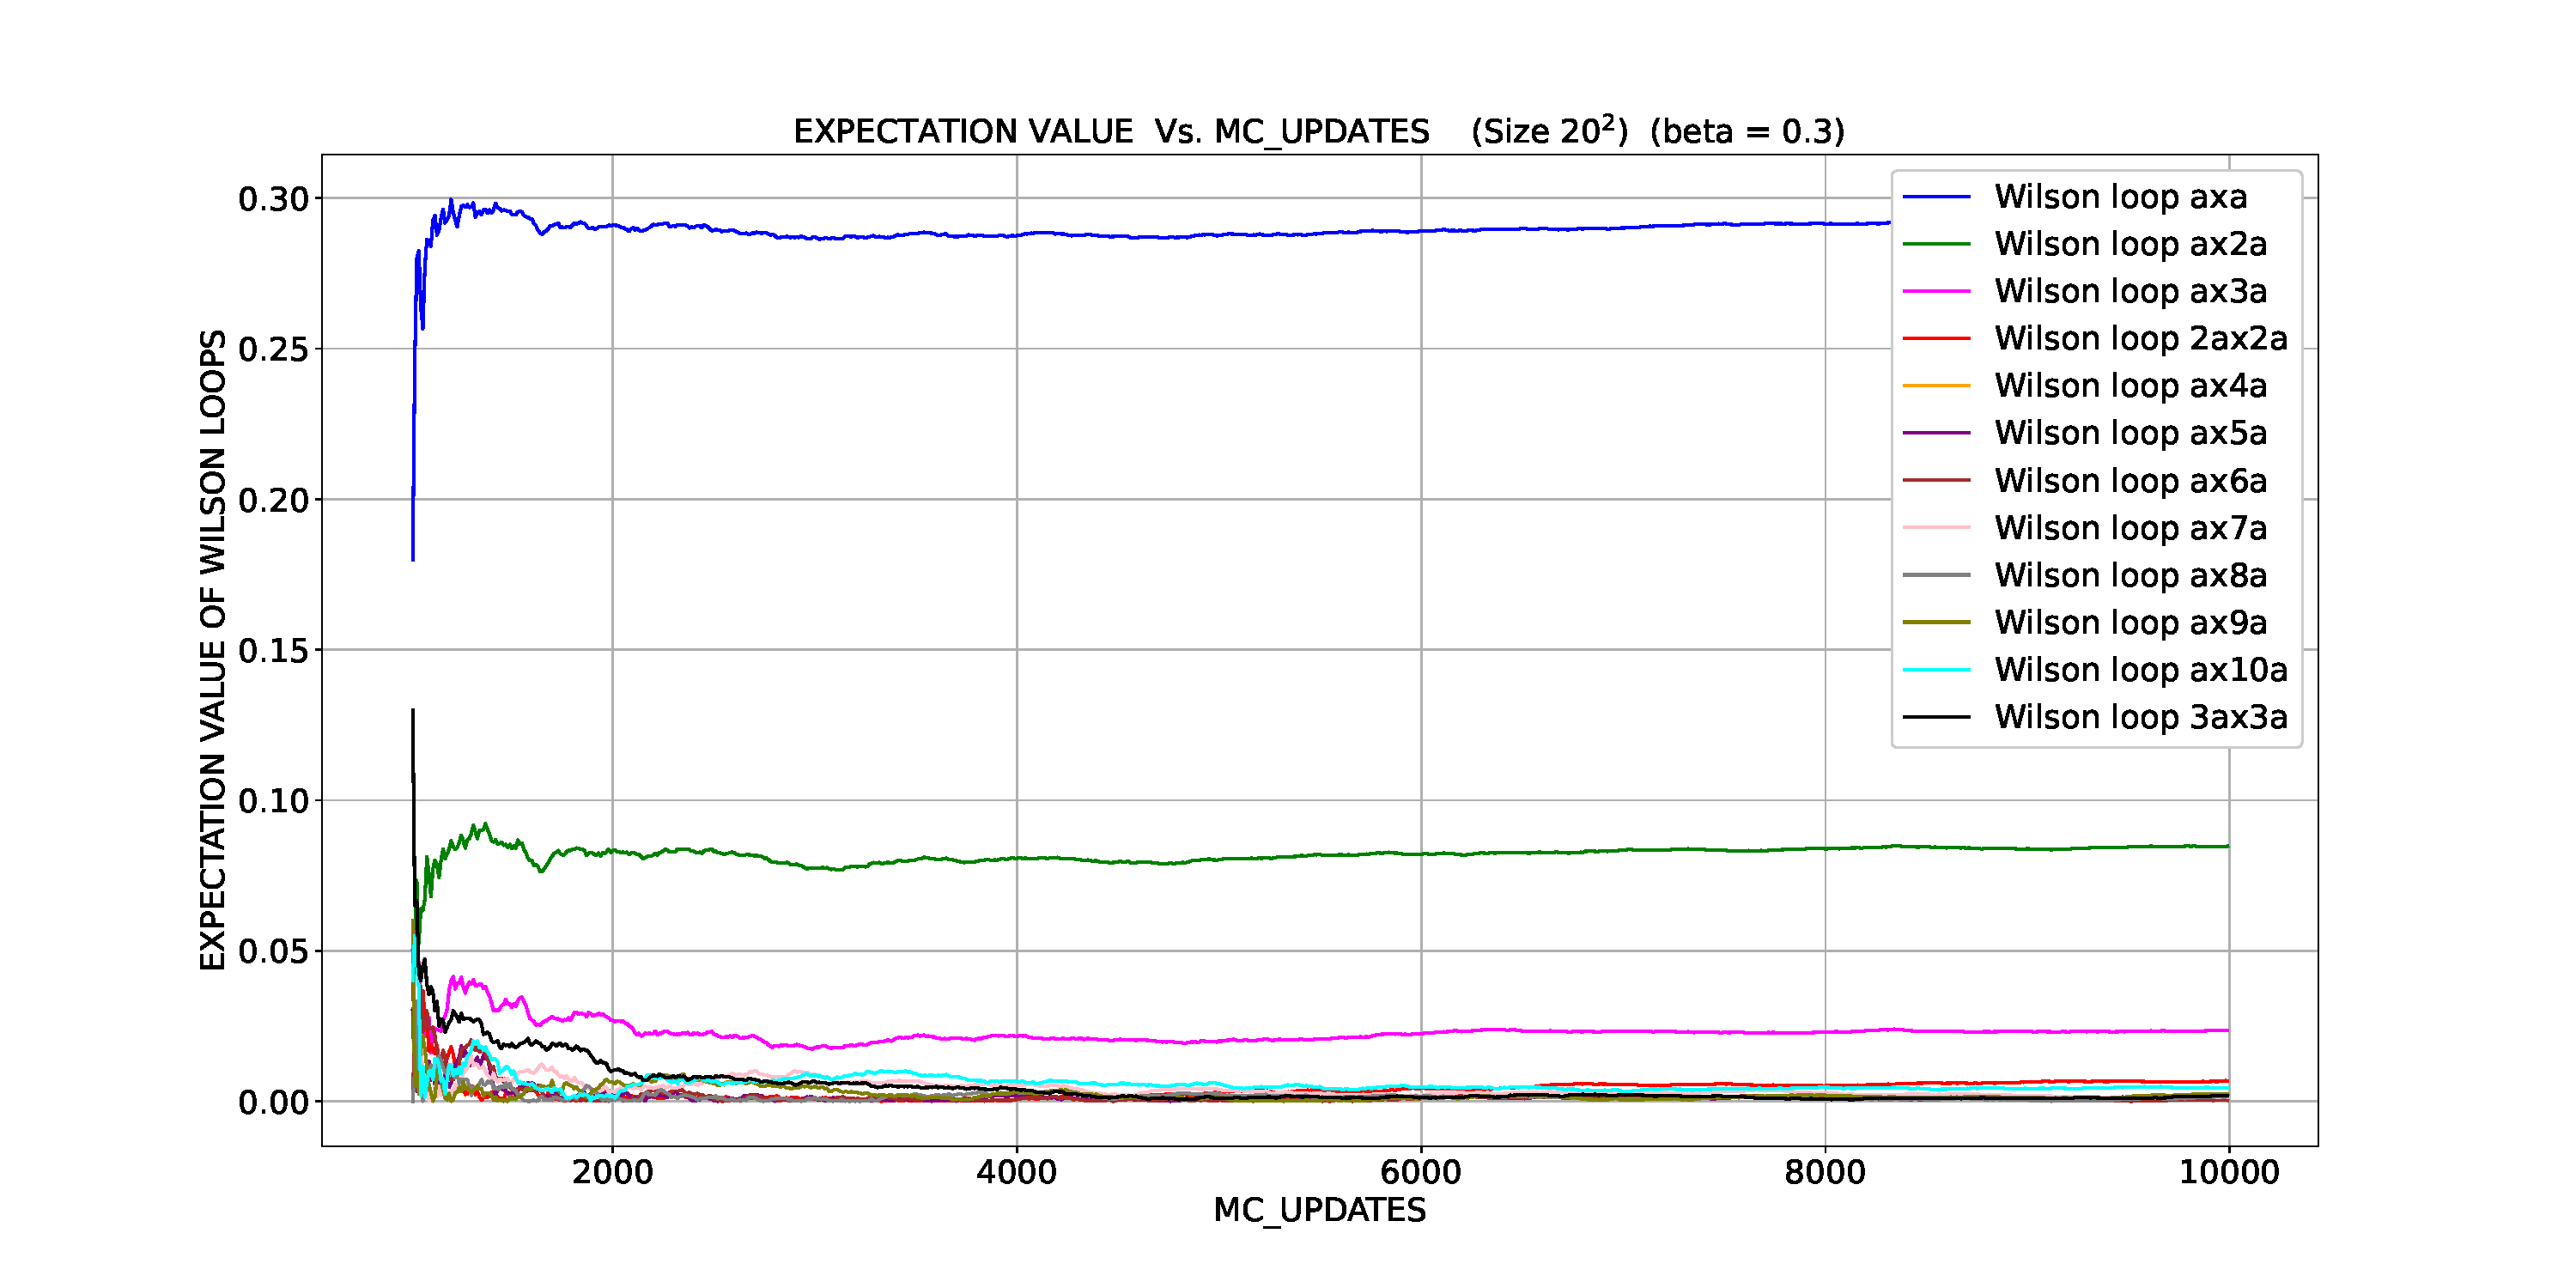
\includegraphics[width=\linewidth]{mcstepsz2.pdf}\\
      {\scriptsize Markov-chain Monte Carlo history (illustration: $\mathbb{Z}_2$ gauge theory in 1+1D)}
    \end{column}
  \end{columns}
\end{frame}

% Slide 11
\begin{frame}{The nucleon two-point function}
  \begin{columns}[c]
    \begin{column}{0.56\textwidth}
      \[ \chi_\alpha(\vect x,t)=\epsilon^{ijk}\,u^i_\alpha\,u^j_\gamma\,[C^{-1}\gamma_5]_{\gamma\delta}\,d^k_\delta \]
      \[ C_{\alpha\beta}(t,\vect p)=a^3\sum_{\vect x}e^{-i\vect p\cdot\vect x}\,\big\langle\chi_\alpha(\vect x,t)\,\bar\chi_\beta(\vect 0,0)\big\rangle \]
      \begin{itemize}
        \item Wick's theorem: two $u$ propagators and one $d$ propagator from the source.
        \item Spectral decomposition, projected with $\Gamma^+=\frac12(1+\gamma_4)$:
      \end{itemize}
      \[ C_{\Gamma^+}(t,\vect p)=|Z(\vect p)|\,\frac{E(\vect p)+m}{E(\vect p)}\,e^{-E(\vect p)t}\,\big[1+\mathcal O\big(e^{-\Delta E\,t}\big)\big] \]
    \end{column}
    \begin{column}{0.42\textwidth}
      \centering
      \begin{tikzpicture}
        \node[inner sep=0] (image) {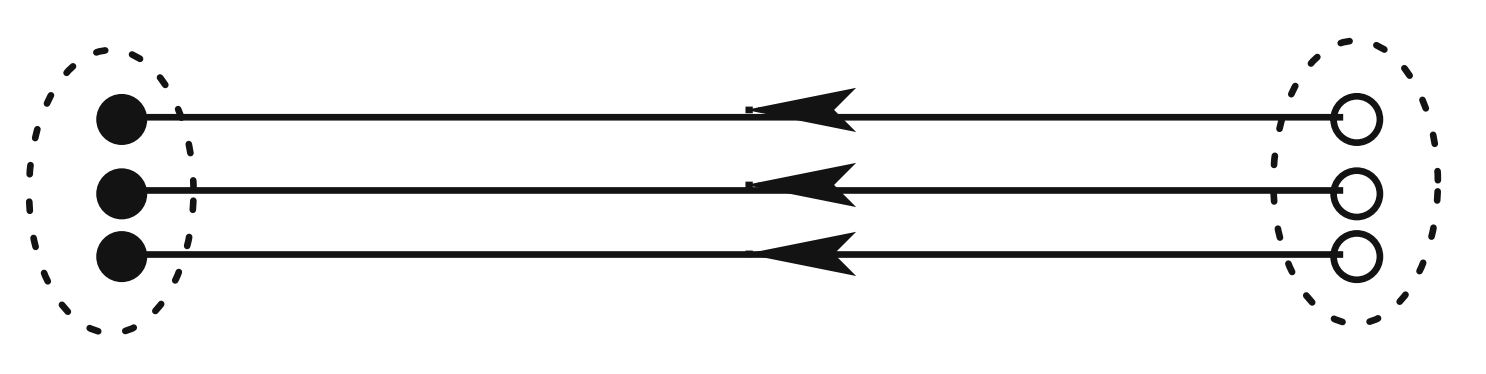
\includegraphics[width=0.85\linewidth]{nucleon_2pt_diagram.png}};
        \node[font=\scriptsize, anchor=south west] at (image.north west) {$(\vect x,t)$};
        \node[font=\scriptsize, anchor=south east] at (image.north east) {$(\vect 0,0)$};
        \node[font=\scriptsize, anchor=north] at (image.south) {$u,\ u,\ d$ propagators $\mathcal{M}^{-1}$};
      \end{tikzpicture}\\[3mm]
      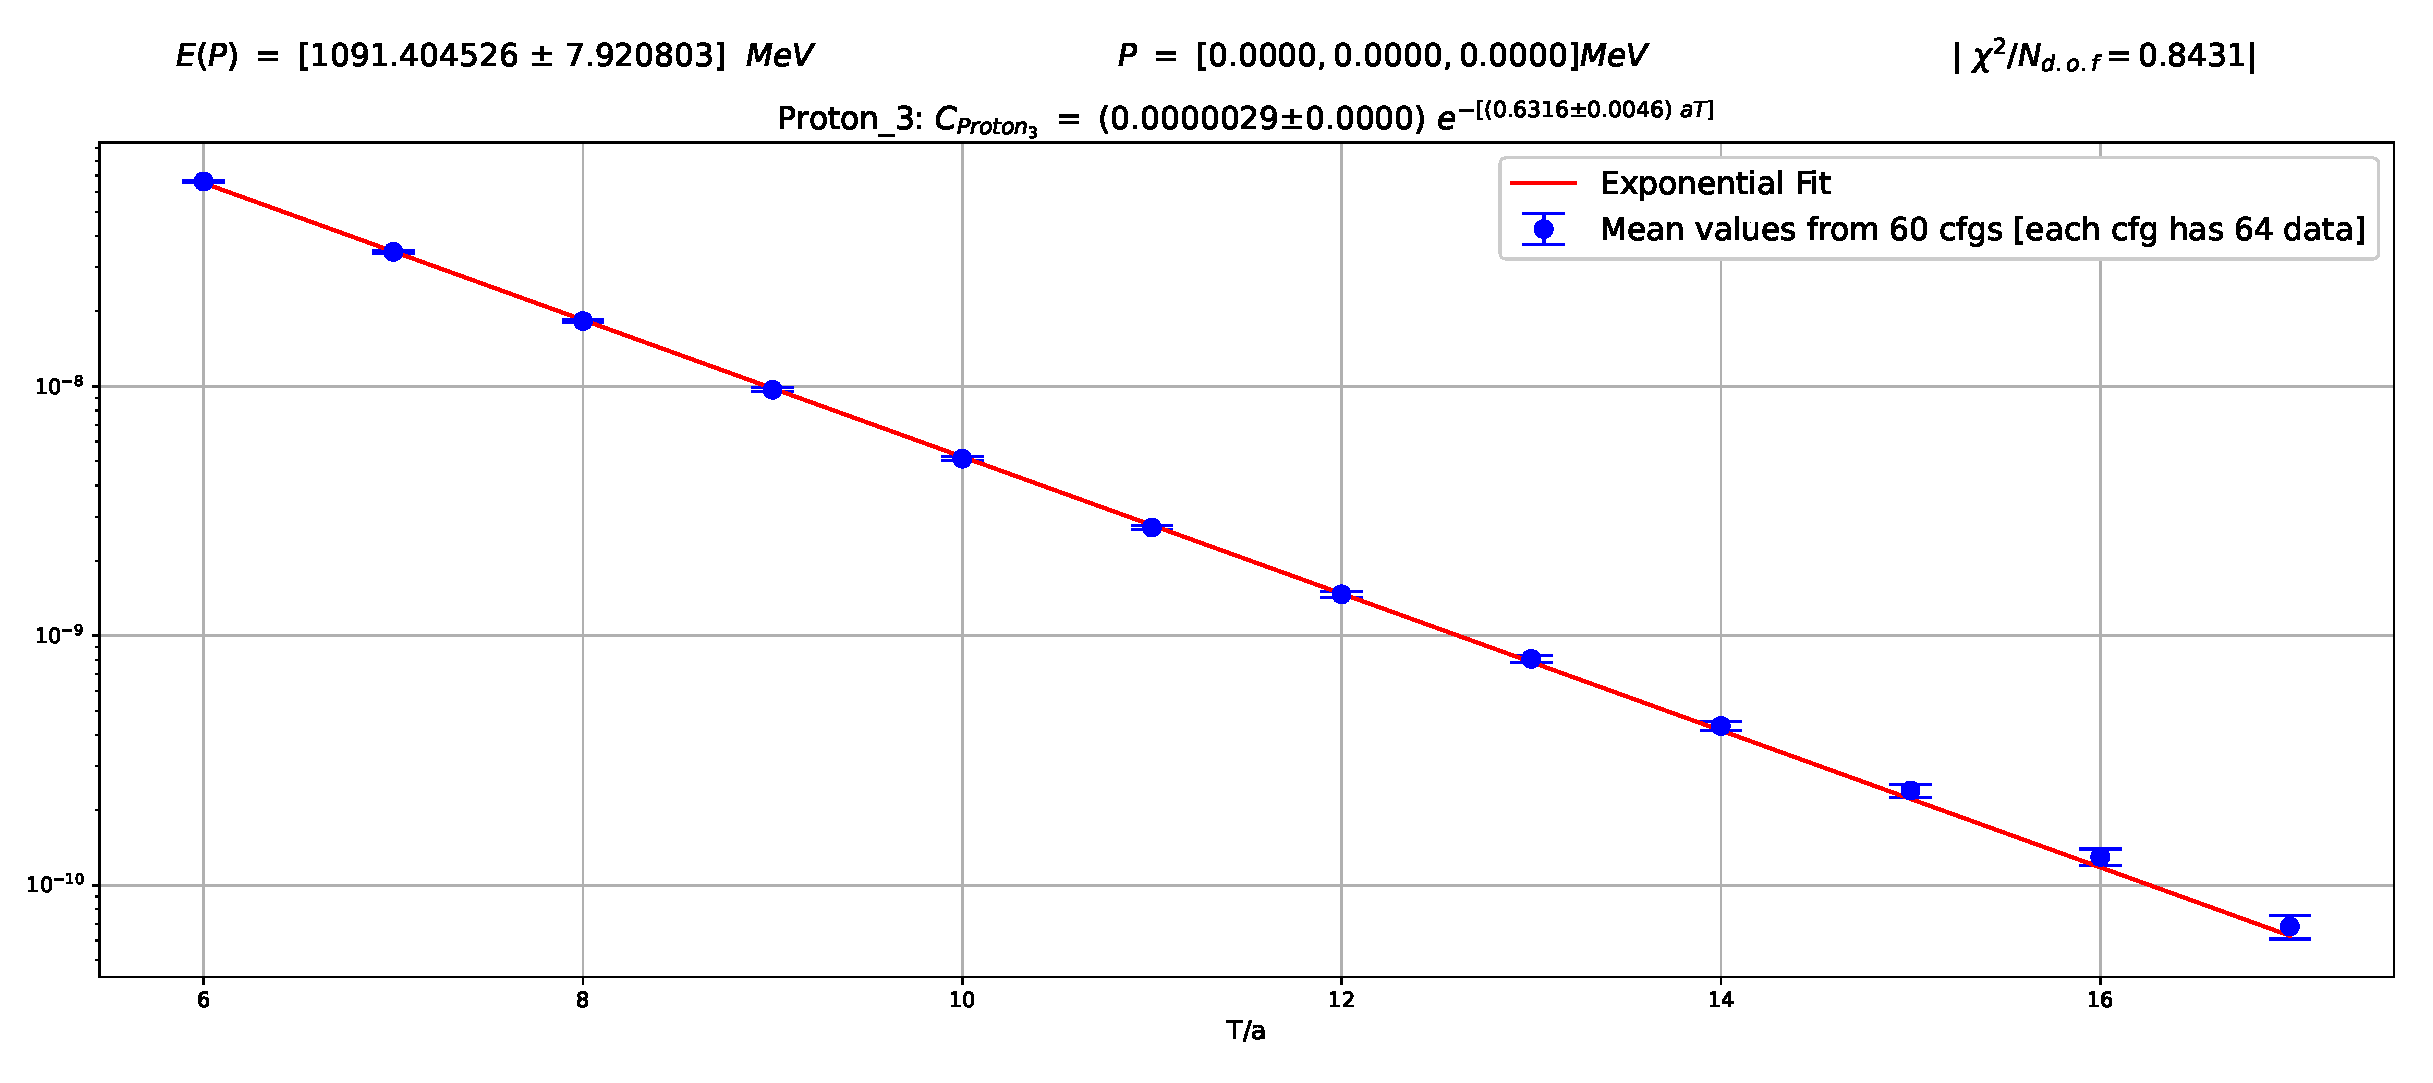
\includegraphics[width=\linewidth]{proton3.eps}\\
      {\scriptsize $C_{\Gamma^+}(t,\vect 0)$ on a different lattice ($32^3\times94$, $a=0.11967$ fm; 2023 study), not the ensemble used in this thesis}
    \end{column}
  \end{columns}
\end{frame}

% Local insertion and complete spectral construction.
\begin{frame}{Nucleon three-point function: source, insertion and sink}
  \small
  \[
  \mathcal O_\Gamma(\vect x_1,\tau)=\bar q(\vect x_1,\tau)\Gamma q(\vect x_1,\tau),
  \qquad 0<\tau<t,\qquad \vect q=\vect p'-\vect p.
  \]
  \begin{align*}
  G(t,\tau;\vect p,\vect p')={}&a^6\sum_{\vect x_2,\vect x_1}
    e^{-i\vect p'\cdot(\vect x_2-\vect x_1)}e^{-i\vect p\cdot\vect x_1}
    \Gamma^{\rm 3pt}_{\beta\alpha}\\
  &\times\big\langle\chi_\alpha(\vect x_2,t)\,
    \mathcal O_\Gamma(\vect x_1,\tau)\,\bar\chi_\beta(\vect 0,0)\big\rangle.
  \end{align*}
  \begin{itemize}
    \item $\bar\chi$ creates nucleon states at the source. The operator acts at $\tau$, and $\chi$ annihilates the states at the sink.
    \item The sink sum projects $\vect p'$. The insertion sum projects the momentum transfer through $e^{i\vect q\cdot\vect x_1}$.
    \item $\Gamma$ specifies the inserted quark bilinear. $\Gamma^{\rm 3pt}$ projects the nucleon spin.
    \item The connected contraction inserts the operator on a nucleon quark line. Disconnected quark loops cancel for $u-d$ in the isospin limit.
  \end{itemize}
  \figsrc{Thesis, Lattice QCD methodology, local three-point functions; Lin (2014), Sec. 3.}
\end{frame}

\begin{frame}{Three-point function: complete spectral sum}
  \small
  With relativistic normalization, insert states on both sides of $\mathcal O$:
  \begin{align*}
  G={}&\sum_{n,n'}\sum_{s,s'}
   \frac{e^{-E_{n'}(\vect p')(t-\tau)}e^{-E_n(\vect p)\tau}}
        {4E_{n'}(\vect p')E_n(\vect p)}\,\Gamma^{\rm 3pt}_{\beta\alpha}\\
  &\times\langle\Omega|\chi_\alpha|N_{n'}(\vect p',s')\rangle
   \langle N_{n'}(\vect p',s')|\mathcal O(\vect q)|N_n(\vect p,s)\rangle\\
  &\times\langle N_n(\vect p,s)|\bar\chi_\beta|\Omega\rangle.
  \end{align*}
  \[
  \langle\Omega|\chi_\alpha|N(\vect p,s)\rangle=\sqrt{Z(\vect p)}\,u_\alpha(\vect p,s),
  \quad
  \langle N'|\mathcal O|N\rangle=\bar u(\vect p',s')\mathcal J u(\vect p,s).
  \]
  \begin{itemize}
    \item $n,n'$ include ground and excited states on the source and sink sides.
    \item Both $\tau$ and $t-\tau$ must be large compared with the inverse excitation gaps for ground-state dominance.
  \end{itemize}
  \figsrc{Thesis, Lattice QCD methodology, spectral decomposition; Lin (2014), Eqs. (3.80)--(3.81).}
\end{frame}

\begin{frame}{Forward matrix element and plateau extraction}
  \small
  For $\vect p'=\vect p$, write $E=E(\vect p)$ and $\Lambda(p)=-i\not\!p+\mN$,
  with Euclidean $p=(\vect p,iE)$.
  \begin{align*}
  G_{00}(t,\tau;\vect p,\vect p)
   &=\frac{|Z(\vect p)|e^{-Et}}{4E^2}
     \Tr[\Gamma^{\rm 3pt}\Lambda(p)\mathcal J\Lambda(p)],\\
  C_{00,\Gamma^+}(t,\vect p)
   &=\frac{|Z(\vect p)|e^{-Et}}{2E}\Tr[\Gamma^+\Lambda(p)],
   \qquad\Gamma^+=\frac{1+\gamma_4}{2}.
  \end{align*}
  \[
  R(t,\tau)=\frac{G(t,\tau)}{C_{\Gamma^+}(t)}
    \xrightarrow{\tau,\,t-\tau\to\infty}
  \frac{\Tr[\Gamma^{\rm 3pt}\Lambda(p)\mathcal J\Lambda(p)]}
       {2E\,\Tr[\Gamma^+\Lambda(p)]}.
  \]
  \begin{itemize}
    \item $G_{00}$ and $C_{00}$ denote the ground-state terms. The overlaps and $e^{-Et}$ cancel in their ratio.
    \item The measured ratio approaches a $\tau$-independent plateau. Finite separations retain excited-state contamination.
    \item A sequential-source inversion fixes the sink time, momentum and spin projector while allowing insertion positions to vary.
  \end{itemize}
  \figsrc{Thesis, Lattice QCD methodology, ratio and sequential propagators; Lin (2014).}
\end{frame}

\begin{frame}{Three-point function: skeleton diagram}
  \centering
  \begin{tikzpicture}[>=Stealth,scale=1.0,
      qline/.style={thick,postaction={decorate},decoration={markings,mark=at position 0.55 with {\arrow{Stealth}}}}]
    % time axis
    \draw[->,gray] (-0.6,-2.6) -- (10.2,-2.6) node[right,gray] {$t$};
    \foreach \x/\l in {0/{0 (source)},4.8/{\tau},9.6/{t (sink)}} \draw[gray] (\x,-2.5)--(\x,-2.7) node[below,font=\small] {$\l$};
    % source and sink blobs
    \fill[blue!25,draw=blue!60!black,thick] (0,0) ellipse (0.45 and 1.5);
    \fill[blue!25,draw=blue!60!black,thick] (9.6,0) ellipse (0.45 and 1.5);
    \node[blue!60!black] at (0,-1.9) {$\bar\chi_\beta(\vect 0,0)$};
    \node[blue!60!black] at (9.6,-1.9) {$\chi_\alpha(\vect x_2,t)$};
    % spectator quarks
    \draw[qline] (0.4,0.7) -- (9.2,0.7);
    \draw[qline] (0.4,0.0) -- (9.2,0.0);
    \node[font=\small] at (4.8,1.05) {spectator quarks};
    % active quark through the operator
    \draw[qline,red!70!black] (0.4,-0.7) -- (4.5,-0.7);
    \draw[qline,red!70!black] (5.1,-0.7) -- (9.2,-0.7);
    \node[fill=red!15,draw=red!70!black,thick,circle,inner sep=3pt] at (4.8,-0.7) {$\mathcal O_\Gamma$};
    \node[red!70!black,font=\small] at (2.4,-1.15) {propagator $S(\vect x_1,\tau;0)$};
    \node[red!70!black,font=\small] at (7.2,-1.15) {sequential propagator};
    \draw[gray,dashed] (4.8,-2.5)--(4.8,1.3);
    \node[font=\small] at (4.8,1.6) {$\mathcal O(\vect x_1,\tau)=\bar q\,\Gamma\,q$};
  \end{tikzpicture}
  \figsrc{Existing schematic of the connected contraction; topology as in thesis, Lattice QCD methodology (Lin, 2014).}
  \begin{itemize}\footnotesize
    \item Connected topology: one quark line (red) carries the operator insertion. Sum over operator position $\vect x_1$ at fixed $\tau$ projects the momentum transfer; the sink sum projects $\vect p'$.
    \item For the TMD operator the single vertex is replaced by the non-local $\bar q(0)\,\Gamma\,\mathcal U\,q(\bvec)$ with a staple gauge link (next slide).
  \end{itemize}
\end{frame}

% Slide 13
\begin{frame}{Non-local staple three-point function: what we compute}
  \begin{columns}[c]
    \begin{column}{0.55\textwidth}
      \begin{itemize}
        \item TMD operator: $\bar q(0)\,\Gamma\,\mathcal U[0,\eta v,\eta v+\bvec,\bvec]\,q(\bvec)$: quark separation $\bvec$, staple direction $v$, staple length $\eta|v|$. Both purely spatial, so the operator sits in one time slice.
        \item On the lattice the staple is a step-wise path $\mathcal C^{\rm lat}$:
      \end{itemize}
      \[ \begin{aligned} C^{\rm 3pt}_{\Gamma}(\tau,\vect P;\mathcal C^{\rm lat})=\frac{1}{\hat L^3}\sum_{z}\Gamma^{\rm 3pt}_{\beta\alpha}\big\langle&\chi_\alpha(t_{\rm snk},\vect P)\,O^{\rm lat}_{\Gamma}(\mathcal C^{\rm lat};z,\tau)\\ &\times\bar\chi_\beta(t_{\rm src},\vect P)\big\rangle \end{aligned} \]
      \[ R_{\Gamma}(\vect P;\mathcal C^{\rm lat})\equiv\mathrm{plateau}\left[\frac{C^{\rm 3pt}_{\Gamma}(\tau,\vect P;\mathcal C^{\rm lat})}{C^{\rm 2pt}(t_{\rm snk}-t_{\rm src},\vect P)}\right] \]
      \begin{itemize}
        \item Inputs: $R_{\Gamma(n)}$ for $\Gamma=\gamma_1,\gamma_2,\gamma_3,\gamma_4$ (isovector $u-d$).
      \end{itemize}
      {\scriptsize Ensemble: $n_f=2+1$ clover, $32^3\times96$, $a=0.11403$ fm, $\mN a=0.6228(28)$ ($\mN=1077.8(48)$ MeV).}
    \end{column}
    \begin{column}{0.43\textwidth}
      \centering
      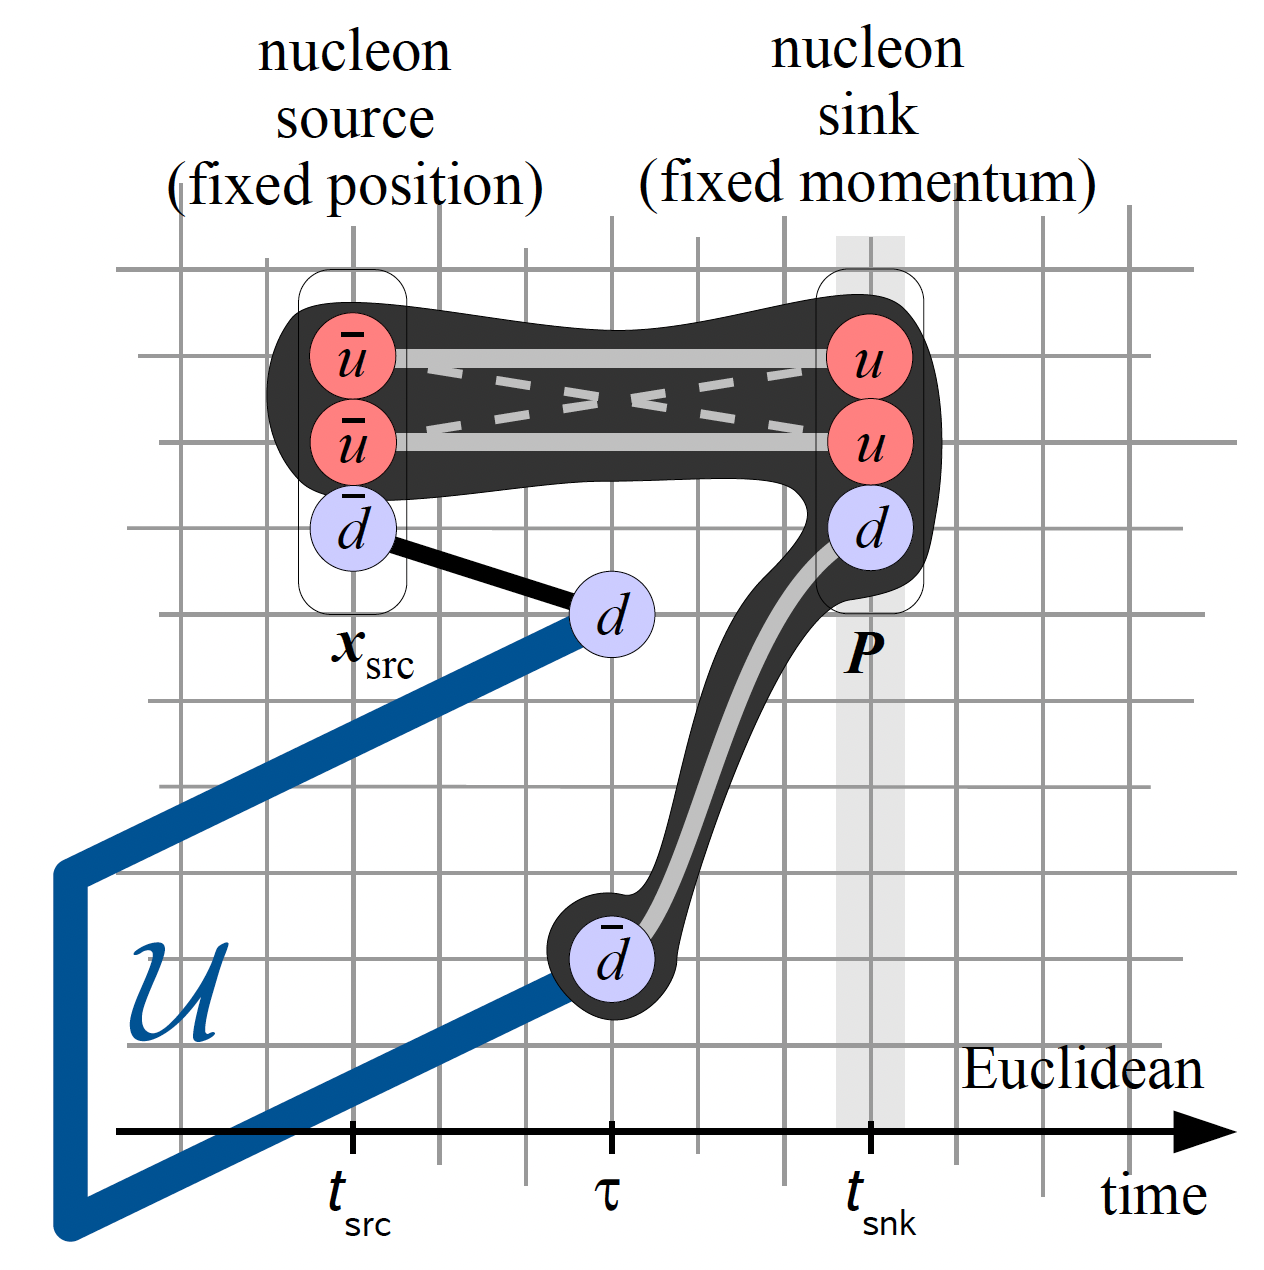
\includegraphics[width=0.9\linewidth]{lattice_3pt_staple_Engelhardt.png}\\
      \figsrc{Figure credit: M.~Engelhardt (NMSU)}
    \end{column}
  \end{columns}
\end{frame}
